\documentclass[12pt]{article}
\usepackage[all, stdclass]{lix}
\usepackage{graphicx}
\usepackage{svg}
\usepackage{pgfplots}
\svgsetup{
  inkscapepath=assets/,  % Path to the directory containing your SVG files
  svgpath=assets/        % Path to the directory containing your SVG files
}
\usepackage{float}
\usepackage{hyperref}
\usepackage{url}
\usepackage{times}
\usepackage{amsmath}
\usepackage{enumitem}
\usepackage{subcaption}
\usepackage{tikz}
\setlist{topsep=0pt, leftmargin=*}
%----------EDIT COVER INFO HERE -----------------%
\def \LOGOPATH {assets/img/birzeit-logo.png}
\def \DEPARTEMENT {Department of Electrical \& Computer Engineering}
\def \COURSENUM {ENEE4113}
\def \COURSENAME {Communications Laboratory}
\def \REPORTTITLE {Phase Modulation}
\def \STUDENTNAME {Mohammad Abu-Shelbaia}
\def \STUDENTID {1200198}
\def \INSTRUCTOR {Dr. Ibrahim Nemer}
\def \ASSISTANT {Eng. Mohammad Al-Battat}
\def \PARTNERAN {Taher Hasan}
\def \PARTNERAID {1191740}
\def \PARTNERBN {Yazan Shrouf}
\def \PARTNERBID {1190145}
\def \REPORTNUM {5}

\begin{document}
\pagenumbering{Roman}

\begin{titlepage}
    \vfill
    \begin{center}
        \includegraphics[width=0.7\textwidth]{\LOGOPATH} \\
        \hfill \\
        \Large{\DEPARTEMENT} \\
        \Large{\COURSENUM\;-\;\COURSENAME} \\
        \vfill
        \textbf{\LARGE{Experiment \#\REPORTNUM}} \\
        \textbf{\LARGE{\REPORTTITLE}}
    \end{center}
    \vfill
    \begin{flushleft}
        \Large{\textbf{Prepared by:}\\ \STUDENTNAME\quad\STUDENTID} \\
        \Large{\textbf{Partners:}\\ 
        \begin{tabular}{@{}l@{\quad}l}
            \PARTNERAN & \PARTNERAID \\
            \PARTNERBN & \PARTNERBID \\
        \end{tabular}} \\
        \Large{\textbf{Instructor:} \INSTRUCTOR} \\
        \Large{\textbf{Assistant:} \ASSISTANT} \\
        \Large{\textbf{Section:} 4}\\
        \LARGE{\textbf{ }}\\
        \LARGE{\textbf{ }}\\
        \LARGE{\textbf{ }}\\
        \Large{\textbf{Date:} \today}\\
    \end{flushleft}
    \vfill
\end{titlepage}
{
    \centering
    \section*{Abstract}
    In this experiment, we study the PM modulation, demodulatiom various techniques, PM spectrum, PM characteristic and how to derive the modulation index. We also study the effect of freqeuncy on modulation spectrum, and the effect of the differnt PLL Loop filter on the demodulated signal.
    \clearpage
}

%--------------- TABLES --------------------------------%
\tableofcontents
\clearpage
\setlength{\parskip}{\baselineskip}%
\listoffigures
\clearpage
\listoftables
\clearpage
\pagenumbering{arabic}
%-------------- CONTENT ---------------------%
\h{Theory}
\hh{Modulation Scheme}
Phase modulation is a part of angle modulation, angle modulation is a technique with constant carrier amplitude and varying phase or time derivative of phase. an FM signal can be expressed as:
\begin{equation}
    s(t) = A_c \cos({\omega}_c t + k_p\times m(t))
\end{equation}
\begin{itemize}
    \item $A_c$ is the carrier amplitude
    \item ${\omega}_c$ is the carrier frequency
    \item $k_p$ is the modulation sensitivity
    \item $m(t)$ is the message signal
\end{itemize}
The instantaneous freqeuncy of the PM Singal is:
\begin{equation}
    f_i = f_c + k_p \times m(t)
\end{equation}
\begin{figure}[H]
    \centering
    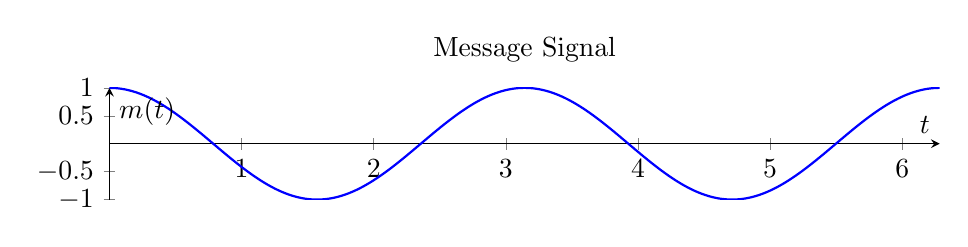
\begin{tikzpicture}
        \begin{axis}[
            width=1\textwidth,
            height=3cm,
            xlabel={$t$},
            ylabel={$m(t)$},
            domain=0:2*pi,
            samples=500,
            axis lines=middle,
            title={Message Signal},
            legend style={at={(0.5,-0.3)},anchor=north},
        ]
        \addplot[blue, thick] {cos(deg(2*x))};
        \end{axis}
    \end{tikzpicture}
    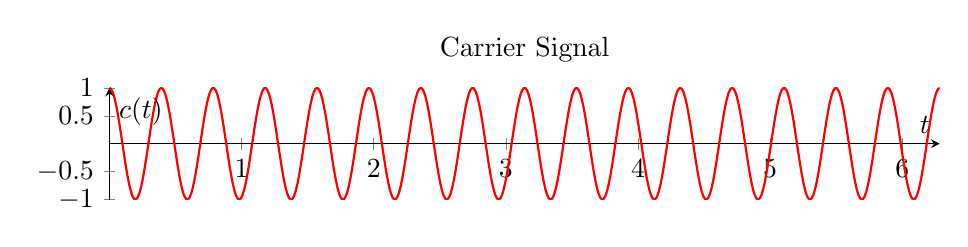
\begin{tikzpicture}
    \begin{axis}[
        width=1\textwidth,
        height=3cm,
        xlabel={$t$},
        ylabel={$c(t)$},
        domain=0:2*pi,
        samples=500,
        axis lines=middle,
        title={Carrier Signal},
        legend style={at={(0.5,-0.3)},anchor=north},
    ]
    \addplot[red, thick] {cos(deg(16*x))};
    \end{axis}
    \end{tikzpicture}
    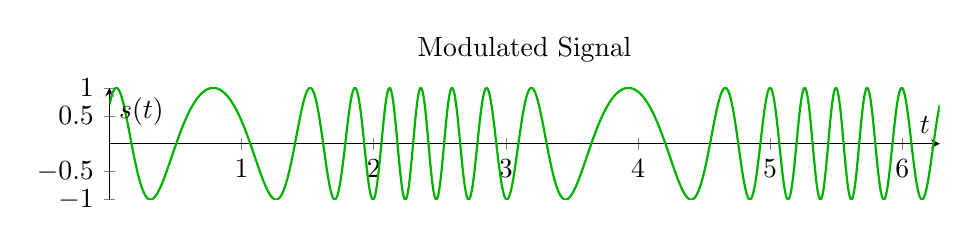
\begin{tikzpicture}
        \begin{axis}[
            width=1\textwidth,
            height=3cm,
            xlabel={$t$},
            ylabel={$s(t)$},
            domain=0:2*pi,
            samples=1000,
            axis lines=middle,
            title={Modulated Signal},
            legend style={at={(0.5,-0.2)},anchor=north},
        ]
        \addplot[green!70!black, thick] {cos(deg(16*x) + 50*2*pi*cos(deg(2*x)))}; % fc = 1, Kf = 64
        \end{axis}
        \end{tikzpicture}
    \caption{Frequency Modulation Scheme}
\end{figure}
\hhh{Modulation}
To generate a PM Singal, we use an oscillator to generate the carrier signal and then modulate the phase of the carrier with the message signal. 
\begin{figure}[H]
    \centering
    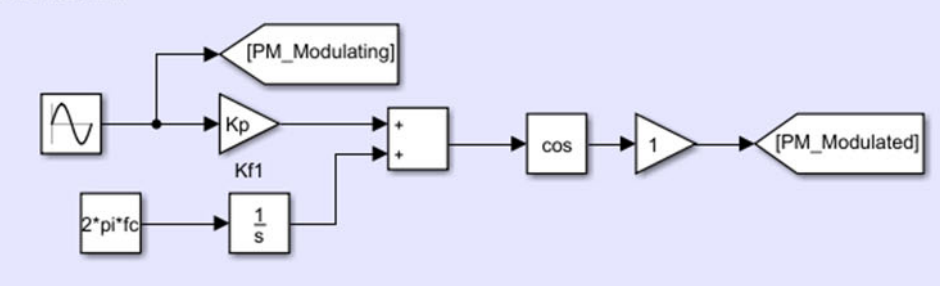
\includegraphics[width=0.8\textwidth]{assets/mod.png}
    \caption{Phase Modulation}
    \cite{Prelab}
\end{figure}

\hhh{Demodulation - Phase Locked Loop}
For demodulation, a common method is the phase-locked loop (PLL) a feedback system that synchronizes the phase of the output signal with the phase of the input signal. The phase detector compares the phase of the input signal with the phase of the output signal and generates an error signal that is used to adjust the phase of the output signal. The output of the phase detector is filtered using a low-pass filter to remove high-frequency components, resulting in a demodulated signal, but the outputs signal is proportional to the derivative of the message singal.
\begin{figure}[H]
    \centering
    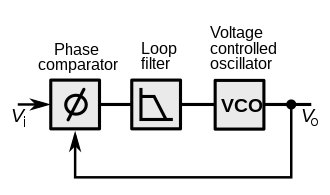
\includegraphics[width=0.5\textwidth]{assets/img/PLL.png}
    \caption{Phase Locked Loop}
    \cite{wikipedia_pll}
\end{figure}
% \hh{Carson's Rule}
% Carson's rule is a rule of thumb that gives the approximate bandwidth of an FM signal. It states that A 98\% power B.W of an FM signal can be estimated by:

% \begin{equation}
%     B_T \approx 2(\beta + 1)f_m
% \end{equation}
% The rule works well when the message signal is continuous. However, it cannot be used when the message contains discontinuities, such as in the case of a square function. \cite{tutorialspoint_fm_modulators}
% \hh{Besel Functions}
% A more accurate expression for the FM signal bandwidth can be obtained using Bessel functions. The FM signal can be expressed as:
% \begin{equation}
%     s(t) = A_c \cos({\omega}_c t + \beta\sin({\omega}_m t))
% \end{equation} 
% where $\beta$ is the modulation index, and ${\omega}_m$ is the message signal frequency. In terms of Bessel functions, the FM signal can be expressed as:
% \begin{equation}
%     s(t) = A_c \sum_{n=-\infty}^{\infty} J_n(\beta) \cos({\omega}_c t + n{\omega}_m t)
% \end{equation}
% To find the bandwidth of the FM signal that achieves a certain percentage of the total power, the following equation can be used:
% \begin{equation}
%     J_0^{2}(\beta) + 2\sum_{n=1}^{m} J_n^{2}(\beta) = p
% \end{equation}
% where $p$ is the percentage of the total power, and $m$ is the number of Bessel functions to be summed, the bandwidth of the FM signal can be calculated using:
% \begin{equation}
%     B_T = 2*m*f_m
% \end{equation}
% \hh{Zero Crossing Decay}
% Zero Crossing is a method to get rid of the carrier spectra,
% and since the spectral components are proportional to the Bessel functions, the zero crossing of the carrier signal occurs when the Bessel function is zero $J_0(\beta) = 0$. 
% \clearpage
\clearpage
\h{Procedure and Data Analysis}
\hh{Modulation}
In this part, we modulated a message signal having 2V VSS and 1kHz frequency over a carrier with 20kHz frequency.
\hhh{Time Domain}
\begin{figure}[H]
    \centering
    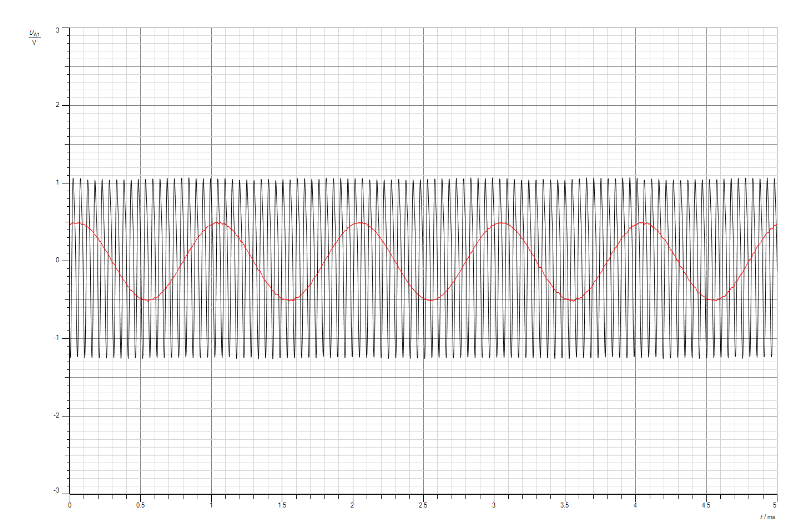
\includegraphics[width=0.7\textwidth]{assets/time_domain.png}
    \caption{Time Domain}
\end{figure}
\hhh{Frequency Domain}
To set the carrier frequency to 20kHz, we set the message signal to 0, so the modulated signal is just the carrier signal.
\begin{equation}
    \begin{aligned}
        s(t) &= A_c \cos({\omega}_c t + k_p\times m(t)) \\
        s(t) &= A_c \cos({\omega}_c t + k_p\times 0)\\
        s(t) &= A_c \cos({\omega}_c t)
    \end{aligned}
\end{equation}
\begin{figure}[H]
    \centering
    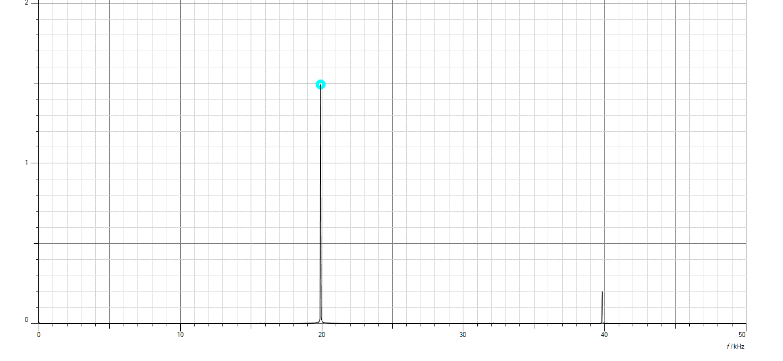
\includegraphics[width=0.7\textwidth]{assets/frequency_domain.png}
    \caption{Frequency Domain}
\end{figure}
From the graph above $f_C = 19.91kHz$, furthermore, we noticed that the modulated signal isn't affected by the amplitude of the message signal, but the frequency of the message signal affects the frequency of the modulated signal.
\hhh{Setting Carrier Frequency}

\hhh{Characteristics of the FM Modulator}
The main Characteristic of the FM modulator is the modulation sensitivity $K_p$, using the instantaneous frequency equation:
\begin{equation}
    f_i = f_c + k_p m(t)
\end{equation}
using a constant amplitude would result
\begin{equation}
    f_i = f_c + k_p \times A_m
\end{equation}
with $f_c$ being the carrier frequency, $k_p$ being the modulation sensetivity, and $A_m$ being the amplitude of the message signal. 
\hh{PM Modulator Characteristic}

\begin{table}[H]
    \resizebox{\textwidth}{!}{%
    \begin{tabular}{|l|l|l|l|l|l|l|l|l|l|l|l|}
    \hline
    Voltage         & -1     & -0.8   & -0.6   & -0.4   & -0.2   & 0      & 0.2 & 0.4   & 0.6   & 0.8   & 1     \\ \hline
    $\Delta t$      & -0.006 & -0.005 & -0.005 & -0.005 & -0.004 & -0.003 & 0   & 0.001 & 0.003 & 0.006 & 0.006 \\ \hline
    $\Delta \phi$ & -119.4 & -99.5  & -99.5  & -99.5  & -79.6  & -59.7  & 0   & 19.9  & 59.7  & 119.4 & 119.4 \\ \hline
    \end{tabular}%
    }
    \caption{PM Modulator Coefficient - $k_p$}
    \label{tab:my-table}
\end{table}
Plotting $\Delta \phi$ over $Voltage$ gives us the modulator coefficient $K_p$ as shown below:
\begin{figure}[H]
    \centering
    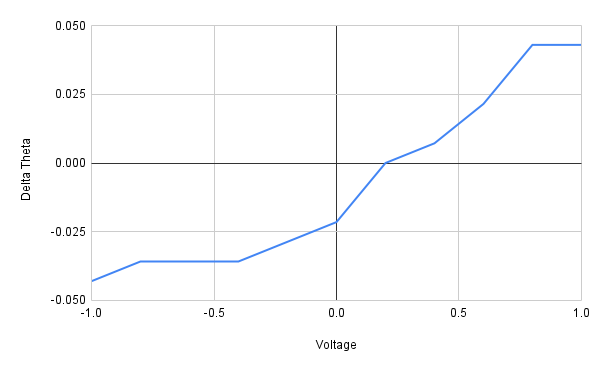
\includegraphics[width=0.7\textwidth]{assets/chart (14).png}
    \caption{Modulator Coefficient - $k_p$}
\end{figure}
Using excel we calculated the slope of the line to be $k_p = 19.61$.
\hh{PM Signal Specturm}
In this part, we studied the effect of Freqeuncy on the modulated singal, by using a constant 2V VSS message with 2 different frequencies 3000Hz and 200Hz and the results were as follows:
\begin{figure}[H]
    \centering
    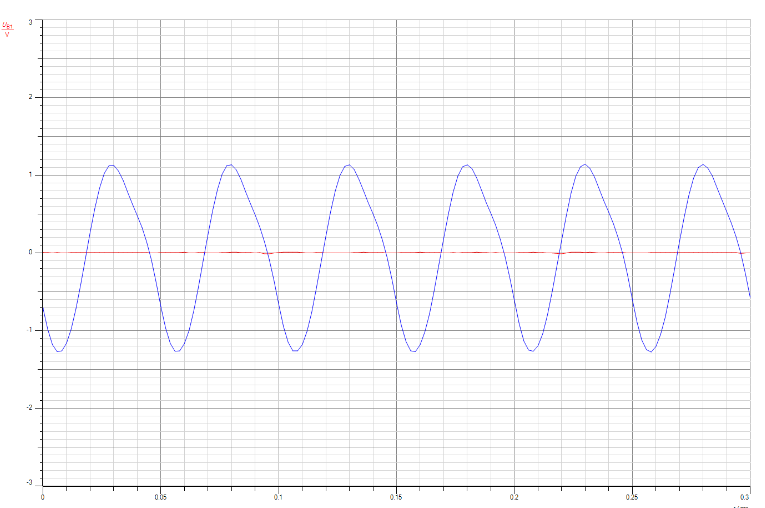
\includegraphics[width=0.7\textwidth]{assets/p2.png}
    \caption{$f_m = 3000Hz$ in time domain}
\end{figure}
\begin{figure}[H]
    \centering
    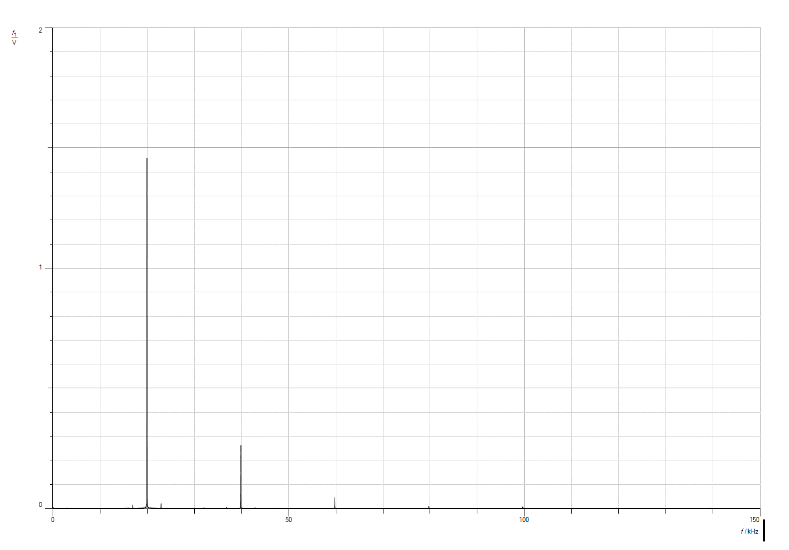
\includegraphics[width=0.7\textwidth]{assets/p1.png}
    \caption{$f_m = 3000Hz$ in frequency domain}
\end{figure}

\begin{figure}[H]
    \centering
    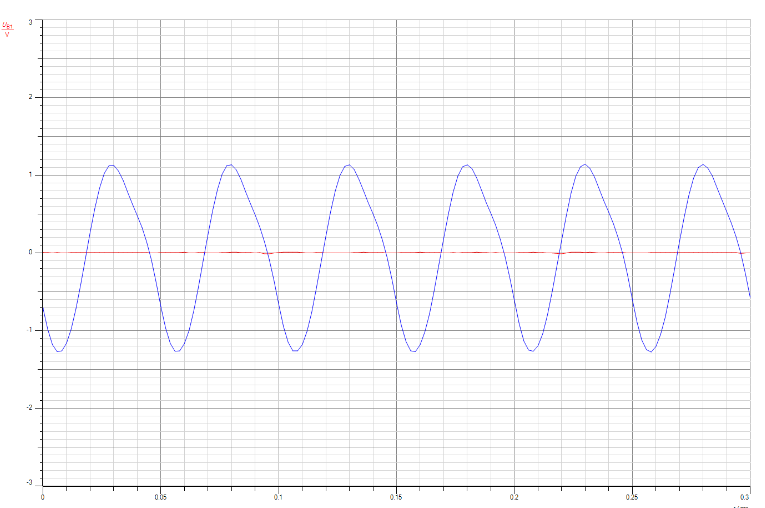
\includegraphics[width=0.7\textwidth]{assets/p2.png}
    \caption{$f_m = 200Hz$ in time domain}
\end{figure}
\begin{figure}[H]
    \centering
    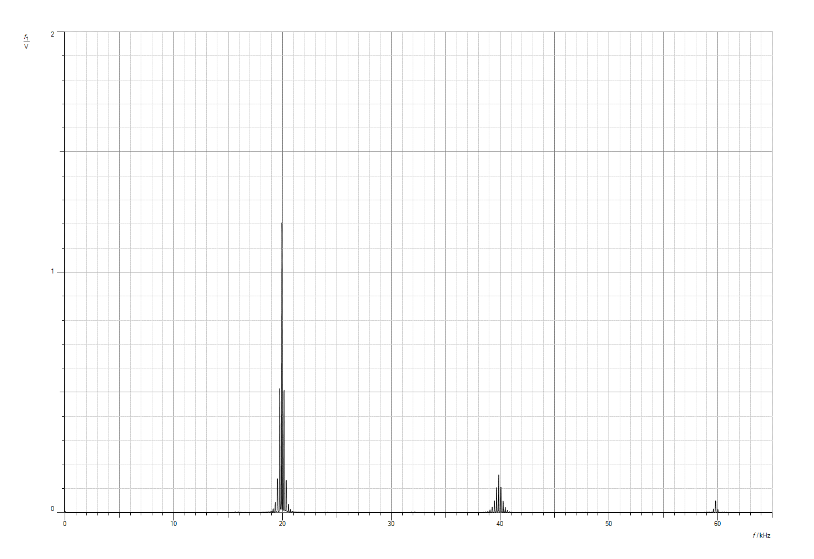
\includegraphics[width=0.7\textwidth]{assets/p4.png}
    \caption{$f_m = 200Hz$ in frequency domain}
\end{figure}
We noticed that the spectrum keeps repeating itself, and the period of repetitions is equal to the frequency of the message signal. And we can't tell the difference between a FM and PM signal from the spectrum.
\hh{Demodulation}
\hhh{Time Domain Demodulatio} 
\begin{figure}[H]
    \centering
    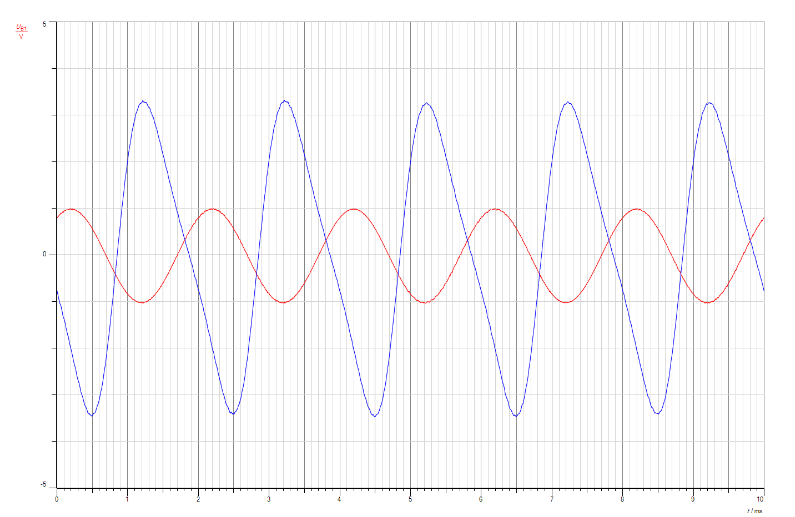
\includegraphics[width=0.7\textwidth]{assets/p5.png}
    \caption{Demodulated Signal in time domain}
\end{figure}
\begin{figure}[H]
    \centering
    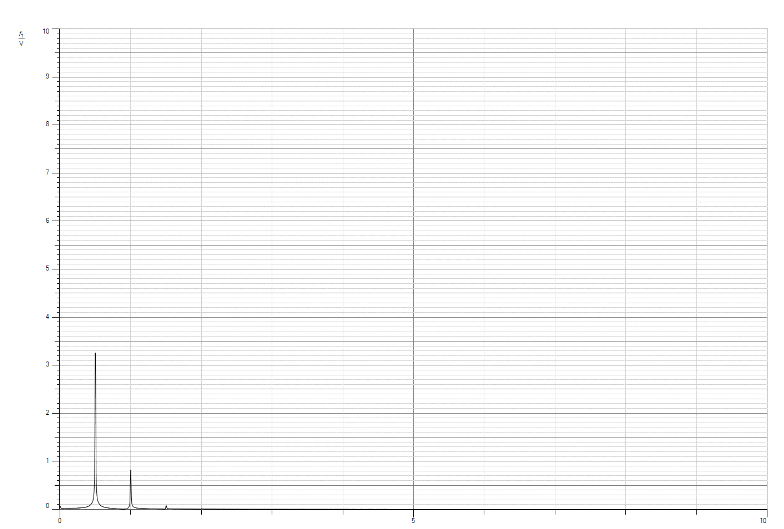
\includegraphics[width=0.7\textwidth]{assets/p6.png}
    \caption{Demodulated Signal in frequency domain}
\end{figure}
We have recoverd the message signal, hence PLL is working with PM, and the demodulated signal is the same as the message signal but with a different amplitude.
\hhh{Studying Loop filters}
% Please add the following required packages to your document preamble:
% \usepackage{graphicx}
\begin{table}[H]
    \resizebox{\textwidth}{!}{%
    \begin{tabular}{|l|r|r|r|r|r|r|}
    \hline
    Frequency & 500   & 1000 & 1500 & 2000 & 3000 & 4000 \\ \hline
    $\tau_1$  & 12.41 & 4.77 & 2.44 & 1.46 & 0.63 & 0.36 \\ \hline
    $\tau_2$  & 3.25  & 2.81 & 2.11 & 1.57 & 0.77 & 0.43 \\ \hline
    \end{tabular}%
    }
    \caption{$\tau_1$, $\tau_2$ vs frequency}
    \label{tab:my-table}
    \end{table}

\begin{figure}[H]
    \centering
    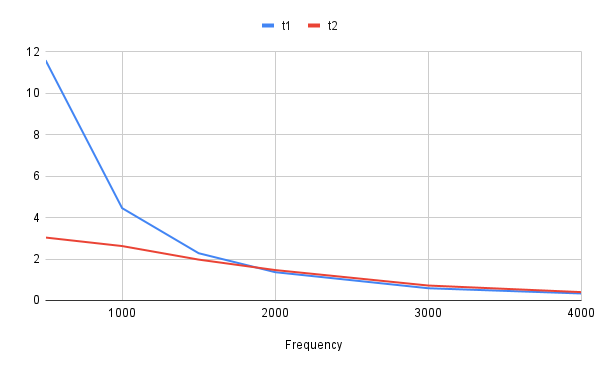
\includegraphics[width=0.7\textwidth]{assets/chart (16).png}
    \caption{$\tau_1$, $\tau_2$ vs frequency}
\end{figure}
We notice that $\tau_1$ and $\tau_2$ are inversely proportional to the frequency, and that $\tau_1$ is always greater than $\tau_2$.
\clearpage
\h{Conclusion}
In conclusion, we have studied the PM modulators and demodulators, the effect of the message signal on the modulated signal, the effect of the frequency on the modulated signal, and Nthe effect of the loop filter on the PLL.
\clearpage
\bibliographystyle{plain}
\bibliography{ref}
\end{document}





